\documentclass[10pt,a4paper]{report}
\usepackage[utf8]{inputenc}
\usepackage[portuguese]{babel}
\usepackage[T1]{fontenc}
\usepackage{amsmath}
\usepackage{amsfonts}
\usepackage{graphicx}
\usepackage{lmodern}
\usepackage{amssymb}
\usepackage{verbatim}
\usepackage{float}
\usepackage{minitoc}
\setcounter{tocdepth}{3}
\usepackage{hyperref}
\title{\LARGE{Segurança e Confiabilidade} \\ \vspace{0.5cm} \normalsize{Resumo}}
\date{}
\renewcommand{\mtctitle}{Conteúdos}

\begin{document}
\maketitle
\tableofcontents

\chapter{Segurança}
\section{Conceitos}
\subsection{Propriedades de Segurança}
As propriedades fundamentais da segurança são:
\begin{itemize}
\item Confidencialidade
\item Integridade
\item Disponibilidade
\item Autenticidade
\item Prestação de contas (accountability)
\end{itemize}
\subsection{Falhas de Segurança}
Uma falha de segurança num sistema procede do seguinte modo:
$$
Ataque + Vulnerabilidade \rightarrow Intus\~ao
$$
\begin{itemize}
\item Um ataque é uma falta intencional maliciosa introduzida no sistema com a intenção de explorar vulnerabilidades
\item Uma vulnerabilidade é uma fraqueza do sistema que o torna sensível a ataques, normalmente não maliciosa, sendo inofensiva sem ataques
\item Uma intrusão é uma falta operacional induzida por meio externo e intencionalmente maliciosa que provoca um estado erróneo no sistema, podendo (ou não) causar uma falha de segurança
\end{itemize}
\subsection{Ataques}
Um ataque pode ser classificado relativamente ao seu propósito:
\begin{itemize}
\item Ataque passivo: tenta-se obter informação existente no sistema sem afetar os seus recursos.  Não requer uma ação explicita contra os mecanismos de proteção ou a integridade dos dados, focando-se na confidencialidade. Alguns exemplos são:
\begin{itemize}
\item Sniffing
\item Traffic analysis
\item Snooping
\item Probing
\end{itemize}
\item Ataque ativo: tenta-se alterar o funcionamento correto do sistema. Consistem em tentativas agressivas de entrar no sistema, para corromper a sua operação e/ou roubar, modificar ou mesmo destruir dados. Alguns exemplos são:
\begin{itemize}
\item Personificação
\item Interposição e alteração
\item Denial of service
\end{itemize}
\end{itemize}
\subsection{Vulnerabilidades}
As vulnerabilidades de um sistema podem tomar forma em deficiências técnicas ou na atitude das pessoas.\\
\\
A defesa contra falhas de segurança baseia-se na prevenção, deteção e recuperação, removendo vulnerabilidades, usando sistemas de deteção de intrusões e repondo o estado antes do ataque.\\
\\
Existem vários princípios de desenho com vista a diminuir potências vulnerabilidades, como o desenho aberto, privilégio mínimo ou isolamento. Um principio em comum é que não se deve confiar apenas em segurança por ocultação, uma vez que mais tarde ou mais cedo, o desenho é divulgado.
\subsubsection{Risco}
O risco é uma métrica composta que leva em consideração o nível de ameaça a que um sistema esta exposto, o seu grau de vulnerabilidade e o impacto financeiro do ataque.
\section{Criptografia}
O propósito da criptografia é a ocultação de informação. Inerentemente, fornece indícios de que se trata de informação sensível, e o seu uso pode ser ilegal. Uma técnica também frequentemente usada é a esteganografia, onde o conteúdo sensível é ocultado dentro de outro conteúdo.
\begin{figure}[H]
\centering
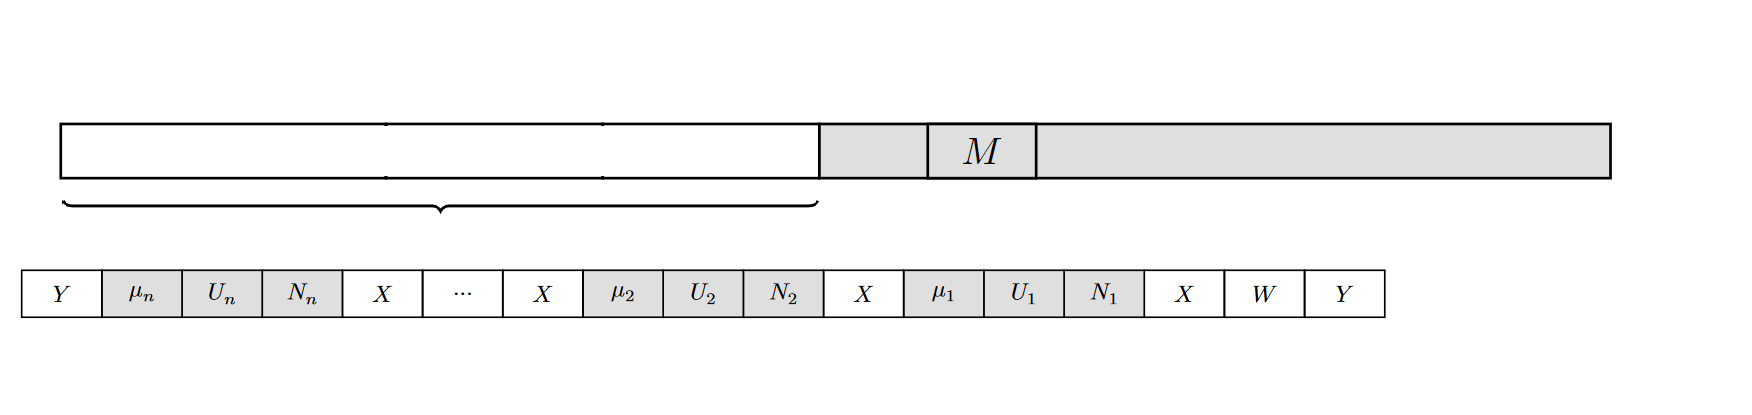
\includegraphics[scale=0.5]{Sem título.png}
\end{figure}
A criptanálise tem como objetivo obter o texto original, obter a chave de cifra/decifra ou obter o algoritmo de cifra usado.
\subsection{Cifras de Substituição}
Existem dois tipos de cifra de substituição:
\begin{itemize}
\item Mono-alfabéticas: usam apenas um alfabeto de substituição, um carácter do alfabeto original é substituído sempre pelo mesmo carácter
\item Poli-alfabéticas: consistem na aplicação sucessiva e cíclica de várias cifras mono-alfabéticas
\end{itemize}
\subsubsection{Cifra de César}
É uma cifra mono-alfabética. Substitui cada letra pela $k$-ésima letra seguinte no alfabeto, $\mod 26$.
\subsubsection{Cifra Vigenère}
É uma cifra poli-alfabética, desde que seja selecionada uma chave com mais que um caráter.
\begin{itemize}
\item É selecionado um conjunto de caracteres, $K$, usado como chave
\item Repete-se a chave em sequência até que a chave seja do tamanho do texto a
ser cifrado
\item Aplica-se à letra do texto em claro a substituição que corresponde à letra correspondente da chave
\end{itemize}
Por exemplo, dado $K = poema$, para cifrar o texto $elesnaosabemq$, usamos a chave $poemapoemapoe$, resultando no texto cifrado $tzienpcwmbtau$. Neste exemplo, dado que a primeira letra original era $e$ e a letra correspondente na chave, $p$ é a 16ª letra do alfabeto, avançamos $e$ 15 letras para a frente (pois $a$ corresponde a 0), resultando em $t$.

\subsection{Cifras de Transposição}
Este tipo de cifra troca a ordem dos caracteres do texto original. Por exemplo, podem ser feitas permutações fixas em blocos com um número constante de caracteres.
\subsection{Conceitos}
\subsubsection{Cifra Perfeita}
Uma cifra diz-se perfeita quando, dado um criptograma $c$, a probabilidade de ele corresponder a um dado texto original $m$ e de ter sido gerado com uma dada chave $k$ é igual à probabilidade de ocorrência do texto $m$. Por exemplo, a cifra de Vernam.\\
\\
O cardinal do espaço de chaves tem de ser igual ou superior ao cardinal do espaço de textos em claro.\\
\\
Surgem algumas dificuldades, como:
\begin{itemize}
\item Tem de ser usada uma chave diferente para cada texto
\item O comprimento das chaves tem de ser igual ou superior ao dos textos
\item As chaves não são memorizáveis
\end{itemize}
\subsubsection{Cifra Segura}
Uma cifra diz-se segura se cumprir o objetivo para que é usada, não permitindo a sua criptanálise em tempo útil e admitindo um investimento tendo em conta a relação custo-benefício.\\
\\
Alguns critérios para avaliar a qualidade de cifras são:
\begin{itemize}
\item Quantidade de secretismo oferecida
\item Dimensão das chaves
\item Propagação de erros
\item Dimensão do criptograma
\end{itemize}
\subsection{Criptografia Simétrica}
Neste tipo de criptografia utiliza-se a mesma chave para cifrar e decifrar. São bastante rápidos, mas necessitam de chaves secretas, cuja gestão pode ser de grande escala.
\subsubsection{Cifra em Blocos}
Atualmente o $Advanced$ $Encryption$ $Stantard$ (AES) é o algoritmo de Rijndael:
\begin{itemize}
\item Recebe como entrada blocos de 128 bits de texto em claro
\item As chaves podem ter 128, 192, 256 bits (quanto maior, mais seguro)
\item Produz blocos de 128 bits de texto cifrado
\item Iterativamente:
\begin{itemize}
\item Cada bloco é dividido em 4 grupos de 4 bytes
\item Um bloco inteiro é modificado em cada iteração
\end{itemize}
\end{itemize}
É rápido e eficiente em CPUs pequenos e grandes.
\begin{figure}[H]
\centering
\includegraphics[scale=0.5]{Sem título1.png}
\end{figure}
\subsubsection{Modos de Cifra em Blocos}
\begin{itemize}
\item $Electronic$ $Code$ $Book$ (ECB)
\begin{itemize}
\item Cifra por blocos independentes
\item Tem uma fraqueza na reprodução de padrões de texto original, dois blocos iguais produzem o mesmo criptograma
\end{itemize}
\begin{figure}[H]
\centering
\includegraphics[scale=0.5]{Sem título37.png}
\end{figure}
\item $Cipher$ $Block$ $Chaining$ (CBC)
\begin{itemize}
\item O texto em claro é XOR com o texto cifrado do bloco anterior antes de ser cifrado
\item Reduz risco de replicação de padrões
\item É usado um $initialization$ $vector$ no primeiro bloco (necessário para decifrar) e é necessário $padding$:  bits para compor blocos inteiros do tamanho requerido pelo algoritmo
\end{itemize}
\begin{figure}[H]
\centering
\includegraphics[scale=0.5]{Sem título33.png}
\end{figure}
\item $Cipher$ $Feedback$ (CFB)
\begin{itemize}
\item Semelhante a CBC, mas a cifra de bloco só é utilizada na direção de cifrar, o que simplifica a sua implementação
\item Também não é necessário $padding$ para um múltiplo do tamanho do bloco porque o algoritmo trabalha com qualquer quantidade de bytes
\end{itemize}
\begin{figure}[H]
\centering
\includegraphics[scale=0.5]{Sem título34.png}
\end{figure}
\item $Output$ $Feedback$ (OFB)
\begin{itemize}
\item Mantém as vantagens to CFB e a mensagem não é utilizada no bloco seguinte, o que implica que as operações de cifra de bloco podem ser feitas antecipadamente permitindo que o XOR seja realizado em paralelo assim que o texto (mensagem ou mensagem cifrada) estiver disponível
\end{itemize}
\begin{figure}[H]
\centering
\includegraphics[scale=0.5]{Sem título35.png}
\end{figure}
\item $Counter$ $Mode$ (CTR)
\begin{itemize}
\item É o modo de cifra padrão no AES
\item É usado um nonce e um contador, que devem ser diferentes em cada operação de cifra
\end{itemize}
\begin{figure}[H]
\centering
\includegraphics[scale=0.5]{Sem título36.png}
\end{figure}
\end{itemize}
\subsubsection{Cifra Contínua}
\begin{figure}[H]
\centering
\includegraphics[scale=0.5]{Sem título2.png}
\end{figure}
\begin{itemize}
\item A cifra de fluxo processa um bit/byte de cada vez através da operação XOR
\item a partir de chave partilhada é produzida uma sequência infinita de bits/bytes aleatórios a que se chama a chave de fluxo ou sequência (keystream)
\item a chave de fluxo é usada uma única vez e portanto é muito difícil a criptanálise
\end{itemize}
Ao cifrar, a chave de fluxo é XOR ao correr do fluxo de texto em claro, bit a bit (ou byte a byte). Ao decifrar, o fluxo cifrado é XOR com a mesma chave de fluxo, o que retorna o fluxo original.\\
\\
É necessário assegurar o secretismo, aleatoriedade e uso único da chave de fluxo, que é gerada nos dois extremos em simultâneo (estão sincronizados).
\subsection{Criptografia Assimétrica}
Neste tipo de criptografia, os dados são cifrados com uma chave pública e decifrados com uma chave privada. São baseados em problemas matemáticos para os quais ainda não foi descoberta uma solução em tempo polinomial. Não são muito eficientes mas têm boa escalabilidade.
\subsubsection{RSA}
Neste algoritmo, o texto em claro é dividido em blocos, que são tratados como um número. As chaves são geradas da seguinte forma:
\begin{itemize}
\item Escolhem-se dois números primos $p$ e $q$
\item Considera-se $n = pq$ e $z = \phi(n) = (p-1)(q-1)$
\item Escolhe-se $e < n$ tal que $e$ é primo com $z$
\item Calcula-se $d$ tal que $ed \mod z = 1$
\item A chave pública é $K_u = (e,n)$ e a chave privada $K_r = (d,n)$
\end{itemize}
Para cifrar calcula-se:
$$
E(K_u,m) = m^e \mod n = c
$$
E para decifrar:
$$
D(K_r,c) = c^d \mod n = m
$$
A criptanálise pode consistir em procura de chaves por força bruta ou ataques temporais, onde se consegue estimar $d$ pelo tempo que demora uma decifração.
\subsubsection{Diffie-Hellman}
Neste algoritmo, o objetivo é obter um número secreto $K$, compartilhado entre $A$ e $B$, mas sem o comunicar em claro.
\begin{itemize}
\item Escolhem-se dois números primos $m$ e $n$ públicos ($n$ grande)
\item $A$ gera um número aleatório $x_a$ e calcula $y_a = m^{x_a} \mod n$
\item $B$ gera um número aleatório $x_b$ e calcula $y_b = m^{x_b} \mod n$
\item $y_a$ e $y_b$ são tornados públicos
\item Cada um calcula $K$ localmente:
$$
K = y_b^{x_a} \mod n = y_a^{x_b} \mod n
$$
\end{itemize}
\subsection{Funções de Síntese}
A síntese ou $digest$ de mensagens tem como objetivo produzir valores de dimensão constante (pequena) a partir de entradas (mensagens, ficheiros, ...) de dimensão variável. Não serve para cifrar/decifrar. Algumas propriedades são:
\begin{itemize}
\item Resistência à descoberta do texto original
\item Resistência à descoberta de um segundo texto original
\item Resistência à colisão
\end{itemize}
Para tornar colisões menos prováveis é necessário usar sínteses de tamanhos razoáveis. O ataque do aniversário é usado para encontrar um par de mensagens que colida. Para sínteses de $n$ bits, é necessário tentar aproximadamente $2^{n/2}$ mensagens.
\subsubsection{MD5}
É um algoritmo que produz uma síntese de 128 bits, no entanto, foram encontradas falhas, pelo que a sua utilização não é recomendada.
\subsubsection{SHA}
Existem várias versões, baseadas no desenho do MD4. Recentemente foi demonstrado que é possível criar uma colisão.
\subsection{Autenticação}
\subsubsection{MAC}
O $Message$ $Authentication$ $Code$ (MAC) usa uma chave simétrica partilhada para autenticar uma mensagem. Pode ser produzido de algumas formas:
\begin{itemize}
\item Cifrar mensagem e síntese da mensagem
\item Cifrar síntese da mensagem
\item Fazer síntese da mensagem concatenada com a chave simétrica (HMAC)
\item Funções chaveadas (último criptograma gerado em modo CBC)
\end{itemize}
\subsubsection{Assinatura}
Uma assinatura digital deve cumprir as seguintes propriedades:
\begin{itemize}
\item Autenticidade
\item Integridade
\item Não-reutilização
\item Não-repudiação
\item Não-forjamento
\end{itemize}
Para criar uma assinatura deve-se cifrar com chave privada a síntese do texto original.
\subsection{Criptografia Híbrida}
É possível juntar a criptografia simétrica com a assimétrica. Para cifrar:
\begin{itemize}
\item Gerar chave secreta aleatória
\item Cifrar texto em claro com chave secreta
\item Cifrar chave secreta com chave pública do destinatário
\end{itemize}
Para cifrar e assinar, o texto é assinado em claro e é cifrado o texto em claro com a assinatura.
\section{Gestão de Chaves Públicas}
Existem dois tipos de chaves públicas:
\begin{itemize}
\item Chaves de longa duração
\begin{itemize}
\item Chaves secretas partilhadas entre dois utilizadores
\item Pares de chave pública/privada
\end{itemize}
\item Chaves de curta duração
\begin{itemize}
\item Chaves de sessão, obtidas de forma automática
\item Mudam-se frequentemente
\end{itemize}
\end{itemize}
\subsection{Distribuição}
A distribuição de chaves públicas pode ser feita de várias formas:
\begin{itemize}
\item Distribuição manual, presencial ou eletronicamente, através de canais alternativos
\item Distribuição embebida, através de browsers, com segurança fraca (usada para importar chaves públicas de autoridades de certificação)
\item Distribuição interativa, no âmbito da execução de protocolos
\item Distribuição ad-hoc, a partir de repositórios ou certificados digitais
\end{itemize}
\subsection{Certificados Digitais}
Um certificado digital contém:
\begin{itemize}
\item Chave pública
\item Identificador do dono da chave
\item Identificação da autoridade de certificação
\item Assinatura digital do certificado efetuada pela Autoridade de certificação (entidade certificadora)
\item Tempo de validade limitado (prazo ou certificados de revogação)
\end{itemize}
Os certificados $X.500$ possuem ainda os algoritmos usados na assinatura, números de série e versão. É possível também definir um $distinguished$ $name$ (DN), composto por uma sequência de $relative$ $distinguished$ $names$ (pares atributo valor), que podem identificar, por exemplo, países ou organizações.
\subsubsection{Certificação}
A validação de um certificado exige a verificação da data de validade, existência de revogação e a validade da assinatura.\\
\\
Uma assinatura de uma entidade certificadora pode ser validada segundo uma cadeia de certificação. Algumas organizações possíveis são:
\begin{itemize}
\item Monopólio (apenas uma raiz confiável)
\item Oligarquia (várias raízes confiáveis)
\item Certificação cruzada
\item Malha
\item Anárquica
\end{itemize}
A infraestrutura de chaves públicas (PKI) inclui autoridades de certificação, interligação entre cadeias de certificação e mecanismos para gerir os certificados.
\subsubsection{Revogação de Certificados}
Um certificado pode ser revogado por diversos motivos, tais como a chave privada (pessoal ou da CA) ser comprometida, ou o utilizador abandonar a organização.\\
\\
Existe um protocolo de pergunta/resposta, $Online$ $Certificate$ $Status$ $Protocol$ (OCSP), que mantém uma lista de certificados revogados. É incluído o ID do certificado, motivo da revogação, assinatura da CA e data de emissão.\\
\\
A distribuição desta lista pode ser integral ou parcial.
\subsubsection{Pretty Good Privacy (PGP)}
É um software de proteção de ficheiros e e-mail, que utiliza o modelo anárquico. Utiliza criptografia híbrida, baseada em chave pública para trocar informações de controlo (RSA) e chaves de sessão para trocar dados (IDEA).\\
\\
Existe um ficheiro onde é guardada a chave privada (cifrado com chave secreta) e outro com chaves públicas. A distribuição pode ser feita por ad-hoc ou servidores HTTP/LDAP. A revogação é feita através de um certificado de revogação pelo próprio, pelo que precisa da sua chave privada.
\begin{figure}[H]
\centering
\includegraphics[scale=0.53]{Sem título3.png}
\end{figure}
As condições de autenticidade são:
\begin{itemize}
\item Recebeu certificado de chave pública do dono diretamente
\item Está assinado por alguém em quem confia
\item User ID tem nome completo do dono
\end{itemize}
\section{Gestão de Chaves Secretas}
As chaves secretas são usadas no decorrer da execução de um determinado protocolo e mudam-se frequentemente (cada interação, cada x minutos, etc.), sendo descartadas quando a sessão termina.\\
\\
Diz-se que existe $perfect$ $forward$ $secrecy$ quando a segurança não depende da manutenção do segredo de outras chaves (de longa duração).
\subsection{Chaves de Cifra de Chaves}
Tem como objetivo estabelecer chave de sessão recorrendo a chaves de longa duração. As chaves de longa duração são chaves secretas partilhadas entre as duas partes e a chave de sessão é trocada cifrada com a chave secreta.
\begin{figure}[H]
\centering
\includegraphics[scale=0.4]{Sem título4.png}
\end{figure}
Esta abordagem está sujeita a ataques de repetição. Para lidar com esse tipo de ataques, os participantes devem usar números sequenciais, pelo que devem manter contadores sincronizados. Deve também ser usado um desafio $nonce$.
\subsubsection{Chaves Assimétricas}
Também é possível usar este método recorrendo a criptografia híbrida. A chave de sessão é enviada cifrada com a chave pública do destinatário e é ainda assinada para garantir autenticidade (evitar ataque homem no meio).
\begin{figure}[H]
\centering
\includegraphics[scale=0.4]{Sem título5.png}
\end{figure}
Ainda assim não garante segurança futura perfeita ($perfect$ $forward$ $secrecy$).
\subsection{Diffie-Hellman}
Este algoritmo garante segurança futura perfeita, dado que o cálculo da chave de sessão não envolve nenhuma chave de cifra de chaves, estando apenas sujeito a ataques de homem no meio.
\begin{figure}[H]
\centering
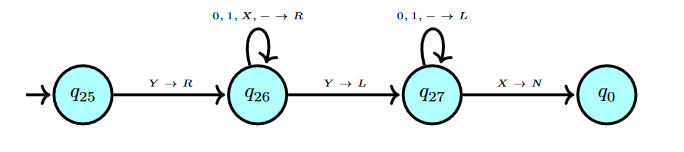
\includegraphics[scale=0.4]{Sem título6.png}
\end{figure}
A solução para este tipo de ataque consiste em validar o mac de cada mensagem, usar desafios-resposta autenticados no final do algoritmo, ou assinar valores públicos (na figura seguinte).
\begin{figure}[H]
\centering
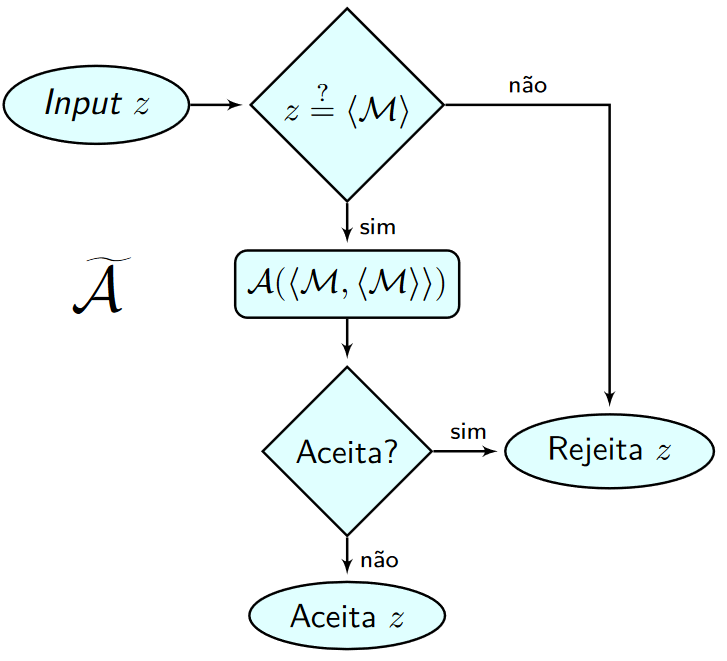
\includegraphics[scale=0.3]{Sem título7.png}
\end{figure}
\subsection{Centros de Distribuição de Chaves (KDCs)}
Um KDC é um mediador em que todos confiam que partilha uma chave simétrica de longa duração com cada participante ($n$ chaves).\\
\\
Tem como vantagem o maior número de chaves partilhadas ($n$ vs. $n(n-1)/2$), no entanto, é um ponto singular de falha e intrusão, um possível ponto de estrangulamento em termos de desempenho e não garante segurança futura perfeita. O funcionamento é o seguinte:
\begin{itemize}
\item Alice contacta o KDC e recebe:
\begin{itemize}
\item[(a)] A chave de sessão cifrada com a chave da Alice
\item[(b)] A chave de sessão + ID da Alice cifradas com a chave de Bob
\end{itemize}
\item Alice envia (b) para o Bob
\end{itemize}
\begin{figure}[H]
\centering
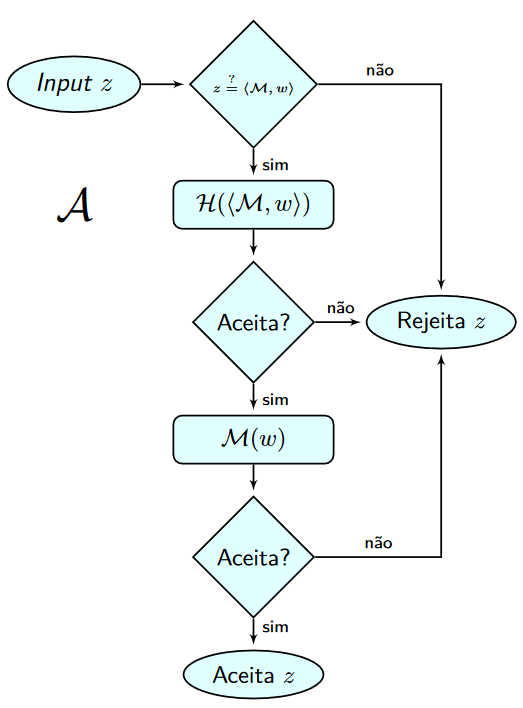
\includegraphics[scale=0.4]{Sem título8.png}
\end{figure}
O problema principal dá-se quando um atacante obtém chave de sessão antiga, consegue personalizar Alice se guardar a mensagem do passo 3.
\section{Autenticação}
Um processo de autenticação permite a um utilizador demonstrar que é a entidade associada a um dado identificador
\subsection{Autenticação Local}
\subsubsection{Autenticação com Passwords}
Este tipo de autenticação é baseado no par <nome, password>. Alguns dos ataques mais comuns são o ataque de dicionário (online ou offline), a reutilização de passwords, rapto de computadores ou engenharia social. O armazenamento de passwords pode ser feito de algumas formas:
\begin{itemize}
\item Texto em claro (não é uma boa solução)
\item Síntese da password
\item Síntese da password + salt
\end{itemize}
A melhor solução é a utilização do salt, pois evita que utilizadores que usem a mesma password tenham o mesmo hash armazenado. Ainda assim, se o adversário capturar o ficheiro e assim tiver acesso aos salts e hashes das passwords, pode usar um programa que experimenta automaticamente diversas passwords até ter sucesso ou uma tabela com estes valores pré-computados.
\subsubsection{Autenticação com Token}
\begin{itemize}
\item Cartão de memória
\begin{itemize}
\item Guarda numa fita magnética ou numa memória interna um segredo e outra informação
\item Tipicamente usa-se em conjunto com uma password
\end{itemize}
\item Cartões/dispositivos com processamento (smart cards / smart token)
\begin{itemize}
\item Têm um processador embebido, capacidade de armazenar dados e alguma forma de interface
\item Suportam/correm algum tipo de protocolo de autenticação seguro com o leitor, sem divulgar as chaves armazenadas
\end{itemize}
\item Passwords Descartáveis
\begin{itemize}
\item É necessário um mecanismo para geração de passwords descartáveis e sincronização por tempo entre cliente/dispositivo e o servidor (password tem validade)
\item Baseado em algoritmos de desafio-resposta (a nova password é baseada num desafio fornecido pelo servidor de autenticação) ou em algoritmos criptográficos (a nova password é baseada na password anterior), como no exemplo seguinte
\end{itemize}
\end{itemize}
No algoritmo Lamport one-time password, é calculado $hash(.....hash(password)...)$ $n$ vezes. O computador conhece $n$ e $hash^n(password)$. Após enviar $n$ ao utilizador, espera receber $x = hash^{n-1}(password)$ verifica se $hash(x) = hash^n(password)$.
\subsubsection{Autenticação Biométrica}
Baseia-se em características físicas estáticas (impressão digital) ou dinâmicas (voz). Funciona recolhendo um padrão associado a uma característica biométrica da pessoa e depois comparando-o mais tarde
\subsection{Autenticação Remota}
A autenticação remota pode ser classificada como unilateral, onde apenas se garante a autenticidade de quem inicia a comunicação ou mútua, onde $A$ prova a sua identidade a $B$, e vice versa.
\subsubsection{Autenticação Unilateral por Partilha de Segredo}
$A$ e $B$ partilham um segredo $K$ e são usados mecanismos de desafio/resposta e marcas de tempo. Por exemplo, Alice envia para Bob: timestamp, Hash(K || timestamp)
\begin{figure}[H]
\centering
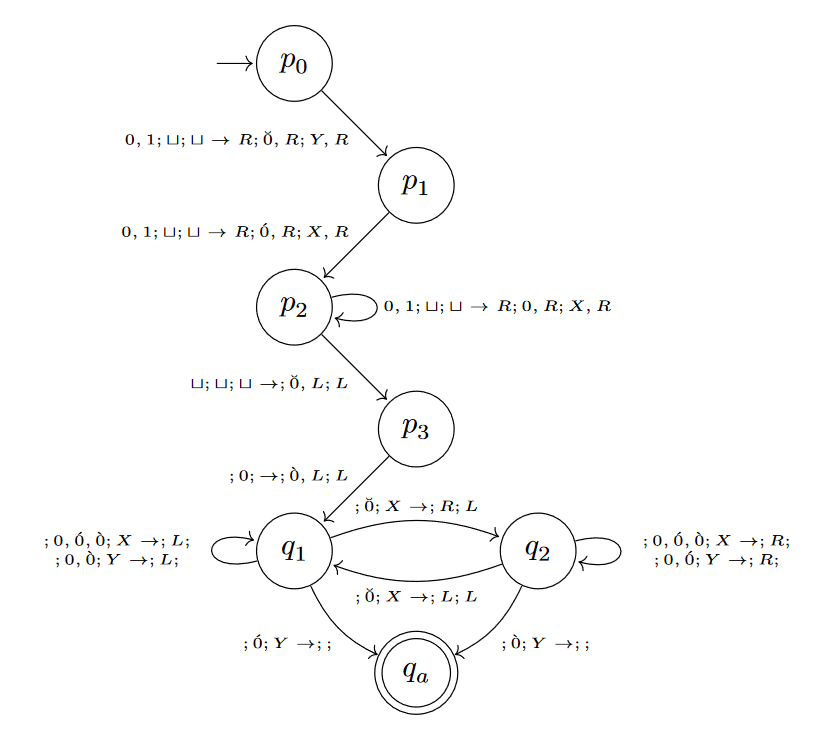
\includegraphics[scale=0.4]{Sem título9.png}
\end{figure}
\subsubsection{Autenticação Unilateral com Chaves Assimétricas}
$B$ conhece a chave pública de $A$, $K_{ua}$. Após uma troca de mensagens, $B$ deve ficar convencido que o seu interlocutor conhece chave privada $K_{ra}$, logo deve ser $A$.
\begin{figure}[H]
\centering
\includegraphics[scale=0.4]{Sem título10.png}
\end{figure}
\subsubsection{Autenticação Mútua com Segredo Partilhado}
\begin{figure}[H]
\centering
\includegraphics[scale=0.4]{Sem título11.png}
\end{figure}
Está sujeito a um ataque de reflexo:
\begin{figure}[H]
\centering
\includegraphics[scale=0.4]{Sem título12.png}
\end{figure}
Existem algumas soluções possíveis:
\begin{itemize}
\item Duas chaves, cada uma usada para uma das direções
\item Desafios com características diferentes (par vs. ímpar)
\item Variante com marca de tempo
\end{itemize}
\subsubsection{Autenticação Mútua com Criptografia Assimétrica}
\begin{figure}[H]
\centering
\includegraphics[scale=0.4]{Sem título13.png}
\end{figure}
Onde $R1$ e $R2$ são $nonces$.
\subsubsection{Autenticação Mediada}
$A$ autentica-se perante $B$ através de um amigo comum, $T$. $A$ partilha um segredo $K_a$ com $T$ e $B$ partilha um segredo $K_b$ com $T$.\\
\\
Alguns métodos de autenticação mediada incluem:
\begin{figure}[H]
\centering
\makebox[\textwidth][c]{\includegraphics[width=1.4\textwidth]{Sem título14.png}}%
\end{figure}
O kerberos segue o seguinte modelo:
\begin{itemize}
\item Entre cliente e servidor kerberos:
\begin{itemize}
\item  O cliente envia uma solicitação de autenticação ao Servidor Kerberos, indicando que deseja obter um Ticket de Autenticação do Cliente (TGT)
\item O Servidor Kerberos autentica o cliente e, se bem-sucedido, envia de volta ao cliente um TGT criptografado
\end{itemize}
\item Entre o cliente e o Ticket Granting Server (TGS):
\begin{itemize}
\item O cliente envia uma solicitação ao TGS, juntamente com o TGT recebido do Servidor Kerberos
\item O TGS verifica o TGT do cliente e, se válido, emite um TSS criptografado, que contém uma chave de sessão para comunicação segura
\end{itemize}
\item Entre o cliente e o servidor:
\begin{itemize}
\item O cliente envia a solicitação original ao Servidor, juntamente com o TSS recebido do TGS.
\item O Servidor verifica o TSS do cliente e, se válido, concede acesso ao serviço solicitado
\end{itemize}
\end{itemize}
\section{Comunicação Segura}
\subsection{Propriedades}
\begin{itemize}
\item Confidencialidade
\item Autenticidade
\item Integridade
\end{itemize}
A concretização destes requisitos geralmente assenta em criptografia a/simétrica.
\subsection{SSL}
SSL é um protocolo que garante comunicação segura sobre o nível transporte. A autenticação pode ser inexistente (para interações anónimas), pode ser unilateral (do lado do servidor) ou mútua.
\subsubsection{Parâmetros}
Cliente e servidor criam um $pre-master-secret$. Os valores são calculador com funções de síntese a partir deste segredo e de $nonces$. Existem duas chaves secretas para MACs e duas chaves para cifra (servidor $\rightarrow$ cliente e cliente $\rightarrow$ servidor).
\subsubsection{Protocolo Record}
Este protocolo é responsável pela comunicação segura, fazendo fragmentação, compressão e cifra e garantindo autenticação e integridade das mensagens. Encapsula protocolos de nível superior, como HTTP, e corre sobre TCP/IP ou outros protocolos de transporte.
\subsubsection{Utilização}
Quando o HTTP corre sobre SSL, é denominado HTTPS. O servidor tem o certificado gerado por uma CA fiável contendo a sua chave pública. O servidor deve provar a sua identidade a pedido do cliente.
\subsection{IPSec}
Trata-se de uma extensão de segurança do protocolo IP. É transparente para aplicações e dá segurança em protocolos de encaminhamento usando a infraestrutura IP existente. Todo o tráfego é tratado de forma indiferenciada.
\subsubsection{Modos}
Existem dois modos possíveis:
\begin{itemize}
\item Modo de transporte
\begin{itemize}
\item Cabeçalho IP original é mantido
\item Utilizado normalmente entre duas entidades finais
\end{itemize}
\item Modo túnel
\begin{itemize}
\item Encapsula o datagrama
\item Usado normalmente quando uma das entidades não é final (routers)
\end{itemize}
\end{itemize}
\subsubsection{Mecanismos}
É possível fazer duas alterações a datagramas IP: cifra do corpo e adição de cabeçalhos extra (MAC).
\begin{itemize}
\item Authentication Header (AH) - Não deve ser usado
\begin{itemize}
\item Autentica o datagrama + (a maioria do) cabeçalho IP + cabeçalho extra AH
\item Garante autenticação da origem e integridade do conteúdo
\item Pode evitar ataques de repetição (inclui contador)
\end{itemize}
\begin{figure}[H]
\centering
\includegraphics[scale=0.3]{Sem título38.png}
\end{figure}
\item Encapsulating Security Payload (ESP)
\begin{itemize}
\item Cifra corpo do datagrama
\item Opcionalmente autentica o corpo do datagrama + cabeçalho ESP
\item Garante integridade do conteúdo
\item Pode evitar ataques de repetição (inclui contador)
\end{itemize}
\begin{figure}[H]
\centering
\includegraphics[scale=0.3]{Sem título39.png}
\end{figure}
\end{itemize}
Estes mecanismos podem ser usados em conjunto:
\begin{figure}[H]
\centering
\includegraphics[scale=0.4]{Sem título15.png}
\end{figure}
\subsection{SSH}
O protocolo SSH (Secure Shell) permite sessões remotas seguras sobre TCP. Utiliza autenticação de ambas as partes e suporta distribuição de chaves manual ou automática.
\begin{figure}[H]
\centering
\includegraphics[scale=0.4]{Sem título16.png}
\end{figure}
\section{Firewalls}
Uma firewall proporciona o ponto único de acesso à rede interna, permitindo definir
regras de controlo de acesso a máquinas/serviços da rede interna e protegendo-a de
várias classes de ataques provenientes da Internet. Deve ser inserida entre a rede interna da organização e a internet.
\begin{itemize}
\item Todo o tráfego do exterior para o interior, e vice versa, deve passar pela firewall
\item Só o tráfego autorizado (definido pela política de segurança) pode passar
\item A firewall deve ser imune a penetrações
\end{itemize}
\subsection{Controlo de Acesso}
\begin{itemize}
\item Controlo dos serviços
\begin{itemize}
\item Determina que serviços podem ser acedidos
\end{itemize}
\item Controlo da direção
\begin{itemize}
\item Determina a direção (de fora para dentro, e de dentro para fora) que um
pedido para um serviço particular pode ser executado
\end{itemize}
\item Controlo do utilizador
\begin{itemize}
\item Determina que utilizadores podem aceder ao serviço
\end{itemize}
\item Controlo de comportamento
\begin{itemize}
\item Controla a forma como são usados determinados serviços
\end{itemize}
\end{itemize}
No entanto, não protege contra ataques que a contornam, ataques provenientes de máquinas internas nem programas/ficheiros infetados com vírus/worms.\\
\\
É possível seguir uma política de segurança:
\begin{itemize}
\item Prudente: tudo o que não é explicitamente permitido não passa
\item Permissiva: tudo o que não é explicitamente negado é permitido
\end{itemize}
\subsection{Packet-Filtering Router}
Este tipo de router aplica um conjunto de regras aos pacotes que chegam e depois reenvia ou descarta os pacotes.\\
\\
Estas regras são ormalmente são baseadas nos cabeçalhos IP e do protocolo nível transporte. Caso não exista nenhuma regra associada ao pacote, aplica-se a política de omissão: descartar ou passar.
\begin{figure}[H]
\centering
\includegraphics[scale=0.6]{Sem título17.png}
\end{figure}
Benefícios:
\begin{itemize}
\item Simplicidade
\item Transparência para com os utilizadores
\item Rápidos
\end{itemize}
Limitações:
\begin{itemize}
\item Não evitam ataques nível aplicacional (não inspecionam o conteúdo das mensagens da aplicação)
\item Não suportam mecanismos avançados de autenticação
\item É relativamente fácil introduzir erros nas regras do filtro
\end{itemize}
Alguns ataques possíveis a este tipo de router incluem:
\begin{itemize}
\item IP address spoofing: o intruso transmite pacotes em que coloca como
endereço IP do emissor um endereço da rede interna.
\begin{itemize}
\item A solução é descartar pacotes provenientes da placa de rede externa com endereços de emissão internos
\end{itemize}
\item Ataques source routing: o emissor especifica no pacote a opção de source
route que indica o caminho a tomar na internet
\begin{itemize}
\item A solução é descartar todos os pacotes com esta opção
\end{itemize}
\item Ataques com fragmentos pequenos: usa-se a fragmentação IP com o
objectivo de se criarem fragmentos muito pequenos, de modo a forçar que os cabeçalhos apareçam em fragmentos distintos.
\begin{itemize}
\item A solução é descartar todos os pacotes em que o protocolo é TCP e o tamanho dos fragmentos é pequeno (1 byte)
\end{itemize}
\end{itemize}
\subsubsection{PFR com Sateful Inspection}
Consiste na utilização de packet-filtering routers que mantêm estado sobre ligações que foram permitidas no passado.
\begin{figure}[H]
\centering
\includegraphics[scale=0.6]{Sem título18.png}
\end{figure}
\subsection{Application-Level Gateway (Application Proxy)}
Trata-se de uma gateway atua na camada de aplicação e suporta aplicações para as quais existe um servidor de proxy. Funciona como representante do servidor interno, agindo como intermediário entre as ligações de rede e analisando o tráfego.
\begin{figure}[H]
\centering
\includegraphics[scale=0.6]{Sem título19.png}
\end{figure}
\begin{itemize}
\item Os utilizadores apenas podem aceder aos servidores proxy, mas nunca se podem ligar diretamente à gateway ou aos servidores da rede interna
\item O servidor de proxy pode ser configurado de forma a suportar apenas o subconjunto de serviços fornecidos pela aplicação que são considerados aceitáveis (seguros), e o resto dos serviços são negados
\end{itemize}
Este método assenta no conceito de uma $Trusted$ $Computing$ $Base$, um subconjunto do sistema que é inerentemente seguro e geralmente usado para executar mecanismos críticos de segurança (eg. firewall).\\
\\
É utilizado um bastion host: uma máquina crítica do ponto de vista de segurança que executa uma versão mais segura do sistema operativo e tem instalados apenas os serviços essenciais.\\
\\
Benefícios:
\begin{itemize}
\item Controlo completo sobre cada serviço: é possível especificar quais os
serviços suportados e com que opções
\item Possibilita formas mais seguras de autenticação e de coleção de
informação de auditoria
\item Mais fácil de configurar e de testar que um PFR
\end{itemize}
Limitações:
\begin{itemize}
\item Requer que os utilizadores se habituem à nova forma de funcionar dos
serviços ou a existência e instalação nas máquinas clientes de software
especializado para acederem a serviços proxy
\item Processamento adicional (overheads) em cada ligação
\end{itemize}
\subsection{Circuit-Level Gateway (Circuit-Level Proxy)}
\begin{figure}[H]
\centering
\includegraphics[scale=0.6]{Sem título20.png}
\end{figure}
A gateway atua na camada de transporte, criando duas ligações (TCP), uma entre ela e a máquina interna e outra entre
ela e a máquina externa e passa o tráfego pela ligação sem fazer qualquer outro processamento.A função de segurança consiste em determinar que ligações é que são permitidas.\\
\\
É usada quando quando os utilizadores internos são de confiança
\subsection{Firewall na Máquina}
É possível criar uma firewall num computador específico (eg. IPtables ou parte do SO), que restringe os pacotes que chegam e saem da máquina.\\
\\
Tem como vantagens as regras de filtragem poderem ser adequadas às necessidades locais, a proteção é feita independentemente da topologia de rede e funciona como um nível extra de proteção.
\subsection{Arquiteturas de Firewalls}
\subsubsection{Inline Firewalls}
\begin{figure}[H]
\centering
\includegraphics[scale=0.6]{Sem título21.png}
\end{figure}
Os computadores são distribuídos por duas (ou mais) zonas de segurança. No exterior (DMZ) são colocados os computadores que necessitam de ser acedidos pela internet (servidores) e no interior os computadores privados da organização.\\
\\
Para conseguir corromper os computadores privados é preciso passar por duas firewalls, mas existe um overhead no acesso á internet nos computadores internos.
\subsubsection{Gateway Simples (Dual Home Gateway)}
\begin{figure}[H]
\centering
\includegraphics[scale=0.6]{Sem título22.png}
\end{figure}
A firewall é constituida por uma máquina com duas ou mais interfaces: uma para o exterior e uma ou mais para redes interiores. Os encaminhadores são opcionais, embora permitam reforçar a segurança uma vez que
podem operar como filtros de pacotes.\\
Vantagens:
\begin{itemize}
\item Simplicidade
\item Economia de recursos
\item Os computadores continuam a ser divididos por duas zonas de segurança,
mas evitamos os atrasos extra nos computadores da rede privada
\end{itemize}
Desvantagens:
\begin{itemize}
\item Comprometimento da gateway-bastião (diretamente exposta a ataques do exterior e do interior)
\item Limitações à localização dos serviços públicos
\end{itemize}
\subsubsection{Screened-Subnet Firewall System}
\begin{figure}[H]
\centering
\includegraphics[scale=0.6]{Sem título23.png}
\end{figure}
Usam-se dois PFR para definir uma zona desmilitarizada, onde são colocados os servidores públicos. O PFR permite apenas mensagens destinadas para o bastion host e o PFR interior permite apenas tráfego cuja origem é o bastion host.\\
\\
Existem duas concretizações diferentes, O single-homed bastion host:
\begin{figure}[H]
\centering
\includegraphics[scale=0.6]{Sem título24.png}
\end{figure}
Onde o acesso às máquinas internas têm de passar pelo PFR e pelo servidor proxy e as regras do packet-filter apenas permitem acesso exterior ao bastion host. Tem a desvantagem de permitir que um intruso escute o tráfego da rede interna se as regras do PFR forem comprometidas.\\
\\
E o dual-homed bastion host:
\begin{figure}[H]
\centering
\includegraphics[scale=0.6]{Sem título25.png}
\end{figure}
Em que o bastion host tem duas interfaces de rede e o re-envio automático de tráfego de uma placa para a outra não é permitido, pelo que os serviços de proxy têm de ser necessariamente usados para que exista acesso à rede interna.\\
\\
O acesso externo ao Information Server pode ser direto ou por intermédio do bastion host.
\subsection{Intrusion Prevention Systems (IPS)}
Extensão aos sistemas de deteção de intrusões (IDS), adicionando-lhes a capacidade de bloquear o tráfego considerado malicioso
\section{Sistemas de Deteção de Intrusões}
Como visto anteriormente, numa arquitetura de segurança tradicional, o PFR tem como função básica a detecção de ataques de personificação de endereço ou outros ataques específicos. O bastion host permite, por exemplo, a execução de formas mais seguras de autenticação e a firewall limita o tráfego entre a DMZ e a rede privada.\\
\\
No entanto podem surgir problemas:
\begin{itemize}
\item Qualquer um dos componentes de software executados na DMZ pode ter um bug de segurança
\item Um ou mais dos mecanismos de segurança não está configurado corretamente
\end{itemize}
Um Sistema de Deteção de Intrusões (SDI) tem como principal função a observação e análise das atividades que ocorrem no sistema, com o objetivo de detetar intrusões. A intrusão pode ser por:
\begin{itemize}
\item Utilizador interno que consegue escalar os seus privilégios
\item Intruso externo que consegue obter acesso a um dos computadores
\end{itemize}
Um SDI pode estar constantemente a monitorizar o sistema de forma a que os ataques sejam detetados em tempo real, ou ser executado esporadicamente
quando existe suspeita de intrusão.
\subsection{Componentes}
Os principais componentes de um SDI são:
\begin{itemize}
\item Sensores
\item Analisador
\item Interface com o utilizador
\item Arquivo de eventos
\end{itemize}
\begin{figure}[H]
\centering
\includegraphics[scale=0.6]{Sem título26.png}
\end{figure}
\subsection{Métodos de Deteção}
\subsubsection{Deteção Baseada no Conhecimento}
\begin{itemize}
\item Compara as atividades observadas com uma lista de padrões/assinaturas de ataque
\item Assume que tudo o que não é conhecido é válido
\item Baixo nível de falsos alarmes (falsos positivos)
\end{itemize}
Vantagens:
\begin{itemize}
\item O número e tipo de eventos a considerar está limitado às atividades descritas nos padrões
\item Os cálculos tendem a ser mais eficientes do que com a deteção baseada no comportamento
\end{itemize}
Desvantagens:
\begin{itemize}
\item Quando surgem novos tipos de ataques, é necessário adicionar novos padrões
\item Adição de padrões poderá ser difícil se não houver uma linguagem standard de especificação
\end{itemize}
\subsubsection{Deteção Baseada no Comportamento}
\begin{itemize}
\item Procura desvios de comportamento dos utilizadores, grupos de utilizadores, servidores, ..., face ao comportamento normal
\item Um modelo é associado a cada utilizador, cuja forma é determinada através da observação do comportamento do utilizador ao longo do tempo (período de aprendizagem)
\item Assume que os desvios são suspeitos
\item Potencialmente um elevado nível de falsos alarmes (falsos positivos)
\end{itemize}
Vantagens:
\begin{itemize}
\item Permite detetar ataques zero-day
\item Podem-se usar técnicas estatísticas e de aprendizagem automática bem conhecidas
\end{itemize}
Desvantagens:
\begin{itemize}
\item As hipóteses sobre os dados recolhidos podem não ser válidas sobre o ponto de vista
estatístico
\item O comportamento de certos utilizadores pode não ser consistente ao longo do tempo
\end{itemize}
\subsection{Detetores de Vulnerabilidades}
Um detetor de vulnerabilidades periodicamente percorre o sistema à procura de vulnerabilidades.\\
\\
Podem ser detetadas através de análise do estado da máquina (programa $x$ versão $y$ tem um bug de segurança conhecido, presença de erros de configuração, ...). Os detetores podem ser:
\begin{itemize}
\item Locais: detetam problemas no sistema onde se está a executa
\item Remotos: Procura problemas de segurança nos sistemas ligados à rede; esta
atividade é conseguida através do envio de pacotes para os serviços de rede
\end{itemize}
Ambos os tipos se complementam.
\subsection{Ação Após Deteção}
Após a deteção e identificação de uma intrusão deve haver uma resposta, que pode ser:
\begin{itemize}
\item Resposta passiva: informa-se o administrador do ataque e espera-se que ele o corrija
\item Resposta ativa: o sistema bloqueia ou afeta o progresso do ataque
\begin{itemize}
\item Iniciar ação contra o intruso (terminar ligação, bloquear com firewall)
\item Alterar o ambiente
\item Recolher mais informação (eg. levar o atacante a tribunal)
\end{itemize}
\end{itemize}

\chapter{Confiabilidade}
\section{Conceitos}
A confiabilidade de um sistema é capacidade do sistema evitar que os seus serviços tenham uma falha mais frequentemente ou com maior severidade do que é
aceitável
\subsection{Terminologia}
\begin{itemize}
\item Sistema: entidade que interage com outras entidades (i.e., outros sistemas)
\item Ambiente: outras entidades que interagem com o sistema de interesse
\item Fronteira do sistema: fronteira entre o sistema e o ambiente
\end{itemize}
Esta ideia aplica-se recursivamente: um sistema é construído a partir de subsistemas, que por sua vez também são formados for subsistemas
\begin{itemize}
\item Requisitos (funcionais, confiabilidade): definem o problema que o sistema resolve
\item Especificação: define o que o sistema deve fazer para cumprir os requisitos
\item Falha: ocorre quando o serviço prestado pelo sistema se desvia do serviço correto
\end{itemize}
\begin{figure}[H]
\centering
\includegraphics[scale=0.6]{Sem título27.png}
\end{figure}
\subsection{Atributos}
\begin{itemize}
\item Fiabilidade: medida em que o serviço se mantém correto ao longo do tempo ($R(t)$ é probabilidade de o sistema estar a funcionar corretamente num dado ambiente operacional até ao instante $t$)
\item Disponibilidade: medida em que o serviço se encontra acessível aos seus utilizadores ($A(t)$ é a probabilidade do sistema estar operacional no instante $t$)
\item Segurança crítica (safety): garantia de ausência de falhas catastróficas para os utilizadores e ambiente
\item Integridade: ausência de alterações incorretas ao sistema
\item Manutenção: capacidade de se poderem proceder a alterações e reparações no sistema
\item Confidencialidade: ausência de divulgação de informação a entidades não autorizadas
\end{itemize}
Notar que um sistema pode ter uma disponibilidade elevada mas uma fiabilidade baixa (e vice versa)
\subsubsection{Segurança Crítica}
Um sistema safety-critical é caracterizado por as falhas terem um impacto muito grande.\\
\\
Na prática, como não se consegue atingir a perfeiçãor, usa-se o risco relacionado com
as perdas médias por unidade de tempo que são observadas no sistema:
$$
risco = \sum_i prb(failure\;i) \times loss(failure\;i)
$$
Onde:
\begin{itemize}
\item $i$ corresponde a todos os tipos de falhas possíveis
\item $prb()$ é a probabilidade de
ocorrência da falha $i$ por unidade de tempo
\item $loss()$ é valor monetário ou
de vidas caso ocorra a falha $i$
\end{itemize}
\subsection{Falhas}
Uma falha ocorre quando:
\begin{itemize}
\item O sistema está num estado erróneo
\item parte do estado erróneo passa para o exterior (torna-se visível na fronteira do sistema)
\end{itemize}
A causa de um erro é uma falta e a consequência é uma falha.
\subsubsection{Classificação de Faltas}
Faltas podem ser classificadas como sendo de paragem, omissão, etc. Podem também ser classificadas quanto á sua manifestação:
\begin{itemize}
\item Falta ativa: uma falta está ativa se causa um erro
\item Falta dormente: a falta existe mas ainda não causou um erro
\item Falta permanente: se a falta existe e mantém-se ao longo do tempo
\item Falta transiente: se a falta aparece esporadicamente
\end{itemize}
\subsection{Melhorar a Confiabilidade}
\begin{itemize}
\item Prevenção de faltas: meios que permitam prevenir a introdução de faltas no sistema
\item Remoção de faltas: meios que possibilitem uma redução do número e severidade de faltas
\item Tolerância a faltas: meios que evitem a falha dos serviços ainda que ocorram faltas
\item Previsão de faltas: meios que facilitem a estimativa das faltas presentes, que irão ocorrer no futuro e as consequências das faltas
\end{itemize}
\subsubsection{Teste de Software}
O teste de software engloba um conjunto muito vasto de técnicas, que consistem em observar o seu comportamento. 
\begin{itemize}
\item Testes estáticos: realizados sem se executar o software
\item Testes dinâmicos: realizados enquanto o programa está em execução
\end{itemize}
Outra terminologia: testes de caixa branca quando se tem acesso ao código e testes de caixa preta se apenas se tem acesso ao executável\\
\\
Existem vários tipos de teste, como testes de unidade, de módulos, integração, etc. Para além disto, podem ser ainda classificados como:
\begin{itemize}
\item Testes funcionais : têm por objetivo garantir que o software faz o que é suposto fazer
\item Testes de segurança : pretende verificar que o software não faz o que não é suposto fazer
\end{itemize}
\subsection{Tolerância a Faltas}
Utiliza técnicas que garantam (com elevada probabilidade) que o sistema não falha ainda que ocorram faltas durante a sua execução.\\
\\
É necessário tirar partido de alguma forma de redundância, que depende do tipo de falta que se pretende tolerar. As principais forma de redundância são:
\begin{itemize}
\item Tempo
\item Informação
\item Componentes
\end{itemize}
\subsection{Arquiteturas Comuns}
\subsubsection{Replicação Ativa}
\begin{figure}[H]
\centering
\includegraphics[scale=0.6]{Sem título28.png}
\end{figure}
É usado um relógio para decidir quando ler valores e produzir resultados.
\begin{itemize}
\item Se ocorrer uma paragem, a outra unidade poderia continuar a fornecer um valor
\item Se for um resultado divergente é necessário parar todo o sistema porque não se sabe qual réplica teve a falha
\item Se ocorrer uma falha na especificação do sistema, em princípio não há nada a fazer se as réplicas forem iguais
\end{itemize}
Existe uma hipótese base que assume que as réplicas falham de modo independente, pelo que se deve assegurar que não ocorrem faltas de modo comum (existe o mesmo bug em ambas, falta de eletricidade, ...).\\
\\
Para que as réplicas produzam os mesmos resultados, existem também duas hipótese face ao determinismo durante a execução:
\begin{itemize}
\item O ambiente é determinista, o que pode ser complicado se os dados forem lidos em momentos diferentes
\item O componente tem uma execução determinista, produzindo os mesmos resultados ao receber as mesmas entradas e partindo do mesmo estado inicial
\end{itemize}
\subsubsection{Ganho de Confiabilidade}
Supondo que ambas as réplicas têm uma probabilidade $p$ de falha por segundo e que o votador nunca falha (otimista).\\
\\
Para falhas arbitrárias (as duas réplicas têm de funcionar corretamente para que votador possa decidir e sistema não pare):
\begin{itemize}
\item Probabilidade de funcionar corretamente: $R = (1 - p) (1 - p) = 1 - 2p + p^2$
\item Probabilidade de falhar: $F = 1 - R = 2p - p^2$
\item MTTF = $1 / (2p - p^2)$
\end{itemize}
Dado que o MTTF de um só componente é $1/p$, não se conseguiu uma melhoria através de replicação, mas tem a vantagem de lidar com faltas arbitrárias.\\
\\
Para faltas de paragem (apenas uma das réplicas têm de funcionar corretamente e dar uma resposta):
\begin{itemize}
\item Probabilidade de funcionar corretamente: $R = (1 - F) = 1 - p^2$
\item Probabilidade de falhar: $F = p*p = p^2$
\item MTTF = $1 / p^2$
\end{itemize}
Conseguiu-se uma melhoria no MTTF através da replicação, tem a vantagem de aumentar a disponibilidade.
\subsubsection{Replicação passíva}
\begin{figure}[H]
\centering
\includegraphics[scale=0.6]{Sem título29.png}
\end{figure}
O comutador ativa a réplica secundária e escolhe a sua saída seguindo a indicação do detetor de falhas. Em geral apenas tolera faltas de paragem.\\
\\
O detetor de faltas monitoriza a réplica primária através de ping, por exemplo, pelo que a deteção pode não ser imediata, mas não há dados de saída incorretos.\\
\\
A réplica secundária opera da seguinte forma:
\begin{itemize}
\item Réplica está parada (cold spare)
\begin{itemize}
\item Não efetua qualquer computação e pode estar desligada
\item Primário guarda estado periodicamente e resultados de operações num log
\item Para que possa substituir o primário, a réplica tem de ser posta em execução e recuperar estado a partir dos dados armazenados
\end{itemize}
\item Réplica está ativa, mas não executa nem tem estado (warm spare)
\begin{itemize}
\item Não executa qualquer operação mas mantém-se pronta para substituir o primário caso seja necessário
\end{itemize}
\item Réplica está ativa e tem estado, mas não executa (hot spare)
\begin{itemize}
\item Não executa qualquer operação mas tem o mesmo estado que o
primário e pode substituí-lo a qualquer momento
\end{itemize}
\end{itemize}
O número de réplicas necessárias para tolerar $f$ faltas depende da classe de faltas consideradas:
\begin{figure}[H]
\centering
\includegraphics[scale=0.6]{Sem título30.png}
\end{figure}
\subsubsection{Previsão de Faltas}
A previsão de faltas é utilizada quando não se consegue evitar/eliminar/tolerar certas faltas, e a ideia é prever a frequência e se os efeitos dessas faltas são aceitáveis. Existem duas atividades na avaliação:
\begin{itemize}
\item Qualitativa que identifica, classifica, e ordena os modos de falha
\item Quantitativa que determina as probabilidades da ocorrência das faltas relevantes e de que forma certos atributos (MTTF) são satisfeitos
\end{itemize}
A injeção de faltas permite por exemplo determinar os efeitos das faltas e a taxa de cobertura dos mecanismos de tolerância a faltas.
\section{Replicação de Informação}
\subsection{Tipos de Erros}
\begin{itemize}
\item Erros isolados: afetam apenas um bit
\item Erros em grupo (burst): afetam um conjunto de bits
\end{itemize}
Os erros isolados são mais simples de detetar mas afetam mais blocos.
\subsection{Códigos de Deteção de Erros}
O objetivo é construir códigos que permitam ao recetor detetar os erros introduzidos durante a transferência de dados pela rede
\begin{itemize}
\item Um código com palavras de $n$ bits tem $2^n$ combinações de 0s e 1s
\item Se o código for estruturado de forma a que apenas um subconjunto das combinações possíveis sejam palavras válidas, então conseguiremos detetar pelo menos alguns dos erros
\end{itemize}
\subsubsection{Distância de Hamming}
A distância de Hamming entre duas palavras de código é o número de bits que as duas palavras diferem (fazer XOR das palavras e contar os 1s).\\
\\
Com $d$ erros isolados transformo (no pior caso) uma palavra na outra se a distância for $d$. Existe sempre deteção se o número de erros for menor que $d$. Algumas características dos códigos são:
\begin{itemize}
\item Distância do código: menor distância de Hamming entre duas quaisquer palavras válidas do código (para detetar $d$ erros preciso dum código com distância $d+1$)
\item Separável: a informação redundante que permite detetar os erros é adicionada ao código original, logo, para uma palavra de código:
$$
bits\;da\;palavra\;de\;código\;=\;bits\;que\;representam\;os\;dados\;originais\;||$$
$$bits\;de\;informação\;redundante
$$
\end{itemize}
\subsubsection{Códigos de Paridade}
Adiciona-se um bit de paridade aos dados originais, permitindo detetar apenas um erro.\\
\\
Pode-se usar paridade ímpar, onde o bit extra tem o valor 0 ou 1 de forma a que o número total de bits a 1 seja ímpar, ou paridade par, onde o total de bits a 1 deve ser par.
\begin{figure}[H]
\centering
\includegraphics[scale=0.8]{Sem título31.png}
\end{figure}
\subsubsection{Checksum}
Códigos de checksum são códigos separáveis, informação que é adicionada aos dados de forma a que se possam detetar erros. Existem alguns tipos de checksum:
\begin{itemize}
\item Checksum de Precisão Simples
\begin{itemize}
\item Adicionam-se os dados originais e ignoram-se os carrys do último bit
\item Podem surgir problemas, ignorar os carry limita a capacidade de deteção do código
\end{itemize}
\item Checksum de Honeywell
\begin{itemize}
\item Junta as palavras de dados duas a duas e depois faz a soma para gerar o checksum
\item Erros no mesmo bit afectam afectam pelo menos dois bits no checksum
\end{itemize}
\item Checksum de Resíduos
\begin{itemize}
\item Semelhante ao checksum de precisão simples, só que os bits de carry são adicionados ao checksum
\item Permite a deteção dum
erro que coloque sempre um bit a um dado valor
\end{itemize}
\end{itemize}
\subsection{Códigos de Correção de Erros}
O objetivo é construir códigos que permitam ao recetor detetar e corrigir os erros
introduzidos. Ao descobrir o bit com erro, basta trocar o seu valor.\\
\\
Para corrigir $d$ erros preciso de um código com distância $2d+1$.
\begin{figure}[H]
\centering
\includegraphics[scale=0.8]{Sem título32.png}
\end{figure}
Nesta situação, existem $2^m$ palavras diferentes de dados numa mensagem e $2^n$ palavras diferentes de código. Garante-se que a correção de um erro é possível se para cada palavra de dados:
\begin{itemize}
\item Associamos uma palavra de código $C$ ($\alpha$)
\item Todas as palavras de código distintas de $C$ em 1 bit são inválidas ($\beta$)
\item Por cada palavra de dados, os subconjuntos $\alpha \cup \beta$ são disjuntos
\end{itemize}
É necessário reservar $n+1$ palavras de código por cada palavra de dados. Logo, dado $m$, deve-se resolver a equação $(m + r + 1) \leq 2^r$ para encontrar $r$ (redundância mínima para correção de um erro).
\begin{figure}[H]
\centering
\makebox[\textwidth][c]{\includegraphics[width=1.5\textwidth]{Sem título40.png}}%
\end{figure}
\begin{figure}[H]
\centering
\includegraphics[scale=0.45]{Sem título41.png}
\end{figure}
\end{document}